% Tamaño de letra.
\documentclass[12pt,titlepage]{article}

%------------------------------ Paquetes ----------------------------------

% Paquetes:

%Para comentarios multilínea.
\usepackage{verbatim}

% Para tener cabecera y pie de página con un estilo personalizado.
\usepackage{fancyhdr}

% Codificación UTF-8
\usepackage[utf8]{inputenc}

% Castellano.
\usepackage[spanish]{babel}

% Tamaño de página y márgenes.
\usepackage[a4paper,headheight=16pt,scale={0.75,0.8},hoffset=0.5cm]{geometry}


% Para poder agregar notas al pie en tablas:
%\usepackage{threeparttable}

% Tipo de letra Helvetica (Arial).
%\usepackage{helvet}
%\renewcommand\familydefault{\sfdefault}

% Gráficos:

% Para incluir imágenes, el siguiente código carga el paquete graphicx
% según se esté generando un archivo dvi o un pdf (con pdflatex).

% Para generar dv.
%\usepackage[dvips]{graphicx}

% Para generar pdf.
\usepackage[pdftex]{graphicx}
\pdfcompresslevel=9

\usepackage{pdfpages}

% Para códigos fuente.
\usepackage{listings}

% Para links.
%\usepackage{hyperref}

\usepackage[section]{placeins}

\usepackage{appendix}
\usepackage{ulem}
\usepackage{float}


%
% Directorio donde están las imagenes.
%
%\newcommand{\imgdir}{includes}
%\graphicspath{{\imgdir/}}

%------------------------------ ~paquetes ---------------------------------

%------------------------- Inicio del documento ---------------------------

\begin{document}

% ---------------------- Encabezado y pie de página -----------------------

% Encabezado: sección a la derecha.
% Pie de página: número de página a la derecha.

\pagestyle{fancy}
\renewcommand{\sectionmark}[1]{\markboth{}{\thesection\ \ #1}}
\lhead{}
\chead{}
\rhead{\rightmark}
\lfoot{}
\cfoot{}
\rfoot{\thepage}

% ---------------------- ~Encabezado y pie de página ----------------------

% -------------------------- Título y autor(es) ---------------------------

\title{???}
\author{}

% -------------------------- ~Título y autor(es) --------------------------

% ------------------------------- Carátula --------------------------------

\begin{titlepage}

\thispagestyle{empty}

% Logo facultad más pie de la figura.
\begin{center}

\includegraphics[scale=0.55]{./logo_caratula}\\
\large{\textsc{Universidad de Buenos Aires}}\\
\large{\textsc{Facultad De Ingeniería}}\\
\small{Año 2011 - 1\textsuperscript{er} Cuatrimestre}
\end{center}

\vfill

% Título central.
\begin{center}

\Large{\underline{\textsc{Introducción a los Sistemas Distribuidos (75.43)}}}

\vfill

% Tabla de integrantes.

\Large{\underline{\textsc{Trabajo Práctico Grupal}}}

\vfill

\Large\underline{Integrantes} \linebreak\linebreak

% Separación entre columnas.
\large\addtolength{\tabcolsep}{-3pt}
% Tres columnas con alineación centrada.
\begin{tabular}{|| c | c | c ||}
  \hline
    \textbf{Apellido, Nombre} & \textbf{Nro. Padrón} & \textbf{E-mail} \\
  \hline
    Mari, Sebastian & 88652 & marisebastian@gmail.com \\
  \hline
    Morandi, Nicolas & XXXX & XXXX@gmail.com \\
  \hline
    Piccoli, Sebastian & XXXX & seba.piccoli@gmail.com \\
  \hline
    Roberts, Karen & 88062 & karenroberts16@gmail.com \\
  \hline
    Wolsdorf, Diego & XXXX & XXXX@gmail.com \\
  \hline
    Ygounet, Guido & 88246 & gygounet@gmail.com \\
  \hline
\end{tabular}
\end{center}

\vfill

\hrule
\vspace{0.2cm}

% Pie de página de la carátula.
\noindent\small{75.43 - Introduccion a los Sistemas Distribuidos}

\end{titlepage}

% ------------------------------- ~Carátula -------------------------------

% -------------------------------- Índice ---------------------------------

% Hago que las páginas se comiencen a contar a partir de aquí.
\setcounter{page}{1}

% Índice.
\tableofcontents
\newpage

% -------------------------------- ~Índice --------------------------------

% ----------------------------- Inicio del tp -----------------------------

\section{Determinación de las subredes}

En base a la topolog\'ia propuesta y utilizando la RFC950, se asignaron las siguientes subredes:

\begin{table}
  \begin{center}
    \begin{tabular}{|l|l|l|l|l|}
      \hline
        \bf{Nombre} & \bf{Hosts} & \bf{Bloque} & \bf{Dirección} & \bf{Máscara} \\
      \hline 
	Moscu		& 247 & 256 & 10.42.5.0     & /24 \\
        Tokyo $^{(*)}$      & 204 & 256 & 10.69.5.0     & /24 \\
        Seul               & 114 & 128 & 10.39.25.128  & /25 \\
        Pekin $^{(*)}$     & 103 & 256 & 192.168.15.0  & /24 \\
        Bagdag $^{(*)}$  & 51  & 64  & 10.39.25.0    & /26 \\
        Singapur $^{(*)}$      & 26  & 32  & 10.69.6.128   & /27 \\
        Taipei              & 21  & 32  & 10.69.6.160   & /27 \\
	Bangkok                & 21  & 32  & 10.39.25.64  & /27 \\       
	Beirut                 & 18  & 32  & 10.69.6.224   & /27 \\
	Kuwait                 & 17  & 32  & 10.69.6.192   & /27 \\
        Yakarta                  & 5   & 8   & 10.27.15.192  & /29 \\
        Damasco             & 2   & 4   & 10.27.15.200  & /30 \\
        Jerusalen                 & 2   & 4   & 10.27.15.204  & /30 \\
        Nueva Deli                 & 2   & 4   & 172.51.5.192  & /30 \\
        Kabul                  & 2   & 4   & 172.51.5.196  & /30 \\
        Katmandu               & 2   & 4   & 172.51.5.200  & /30 \\
        Teheran                 & 2   & 4   & 172.51.5.204  & /30 \\
        Ankara                & 2   & 4   & 135.143.5.0   & /30 \\
        Pionyang               & 2   & 4   & 135.143.5.4   & /30 \\ 
    \hline
    \end{tabular} \\
  \end{center}
  \caption{Asignación de direcciones de red.}
\end{table}
\FloatBarrier

(*): Redes asignadas teniendo en cuenta las direcciones IP fijas de los servidores determinadas por el enunciado. \\

\begin{figure}
  \begin{center}
    \advance\leftskip-3cm
    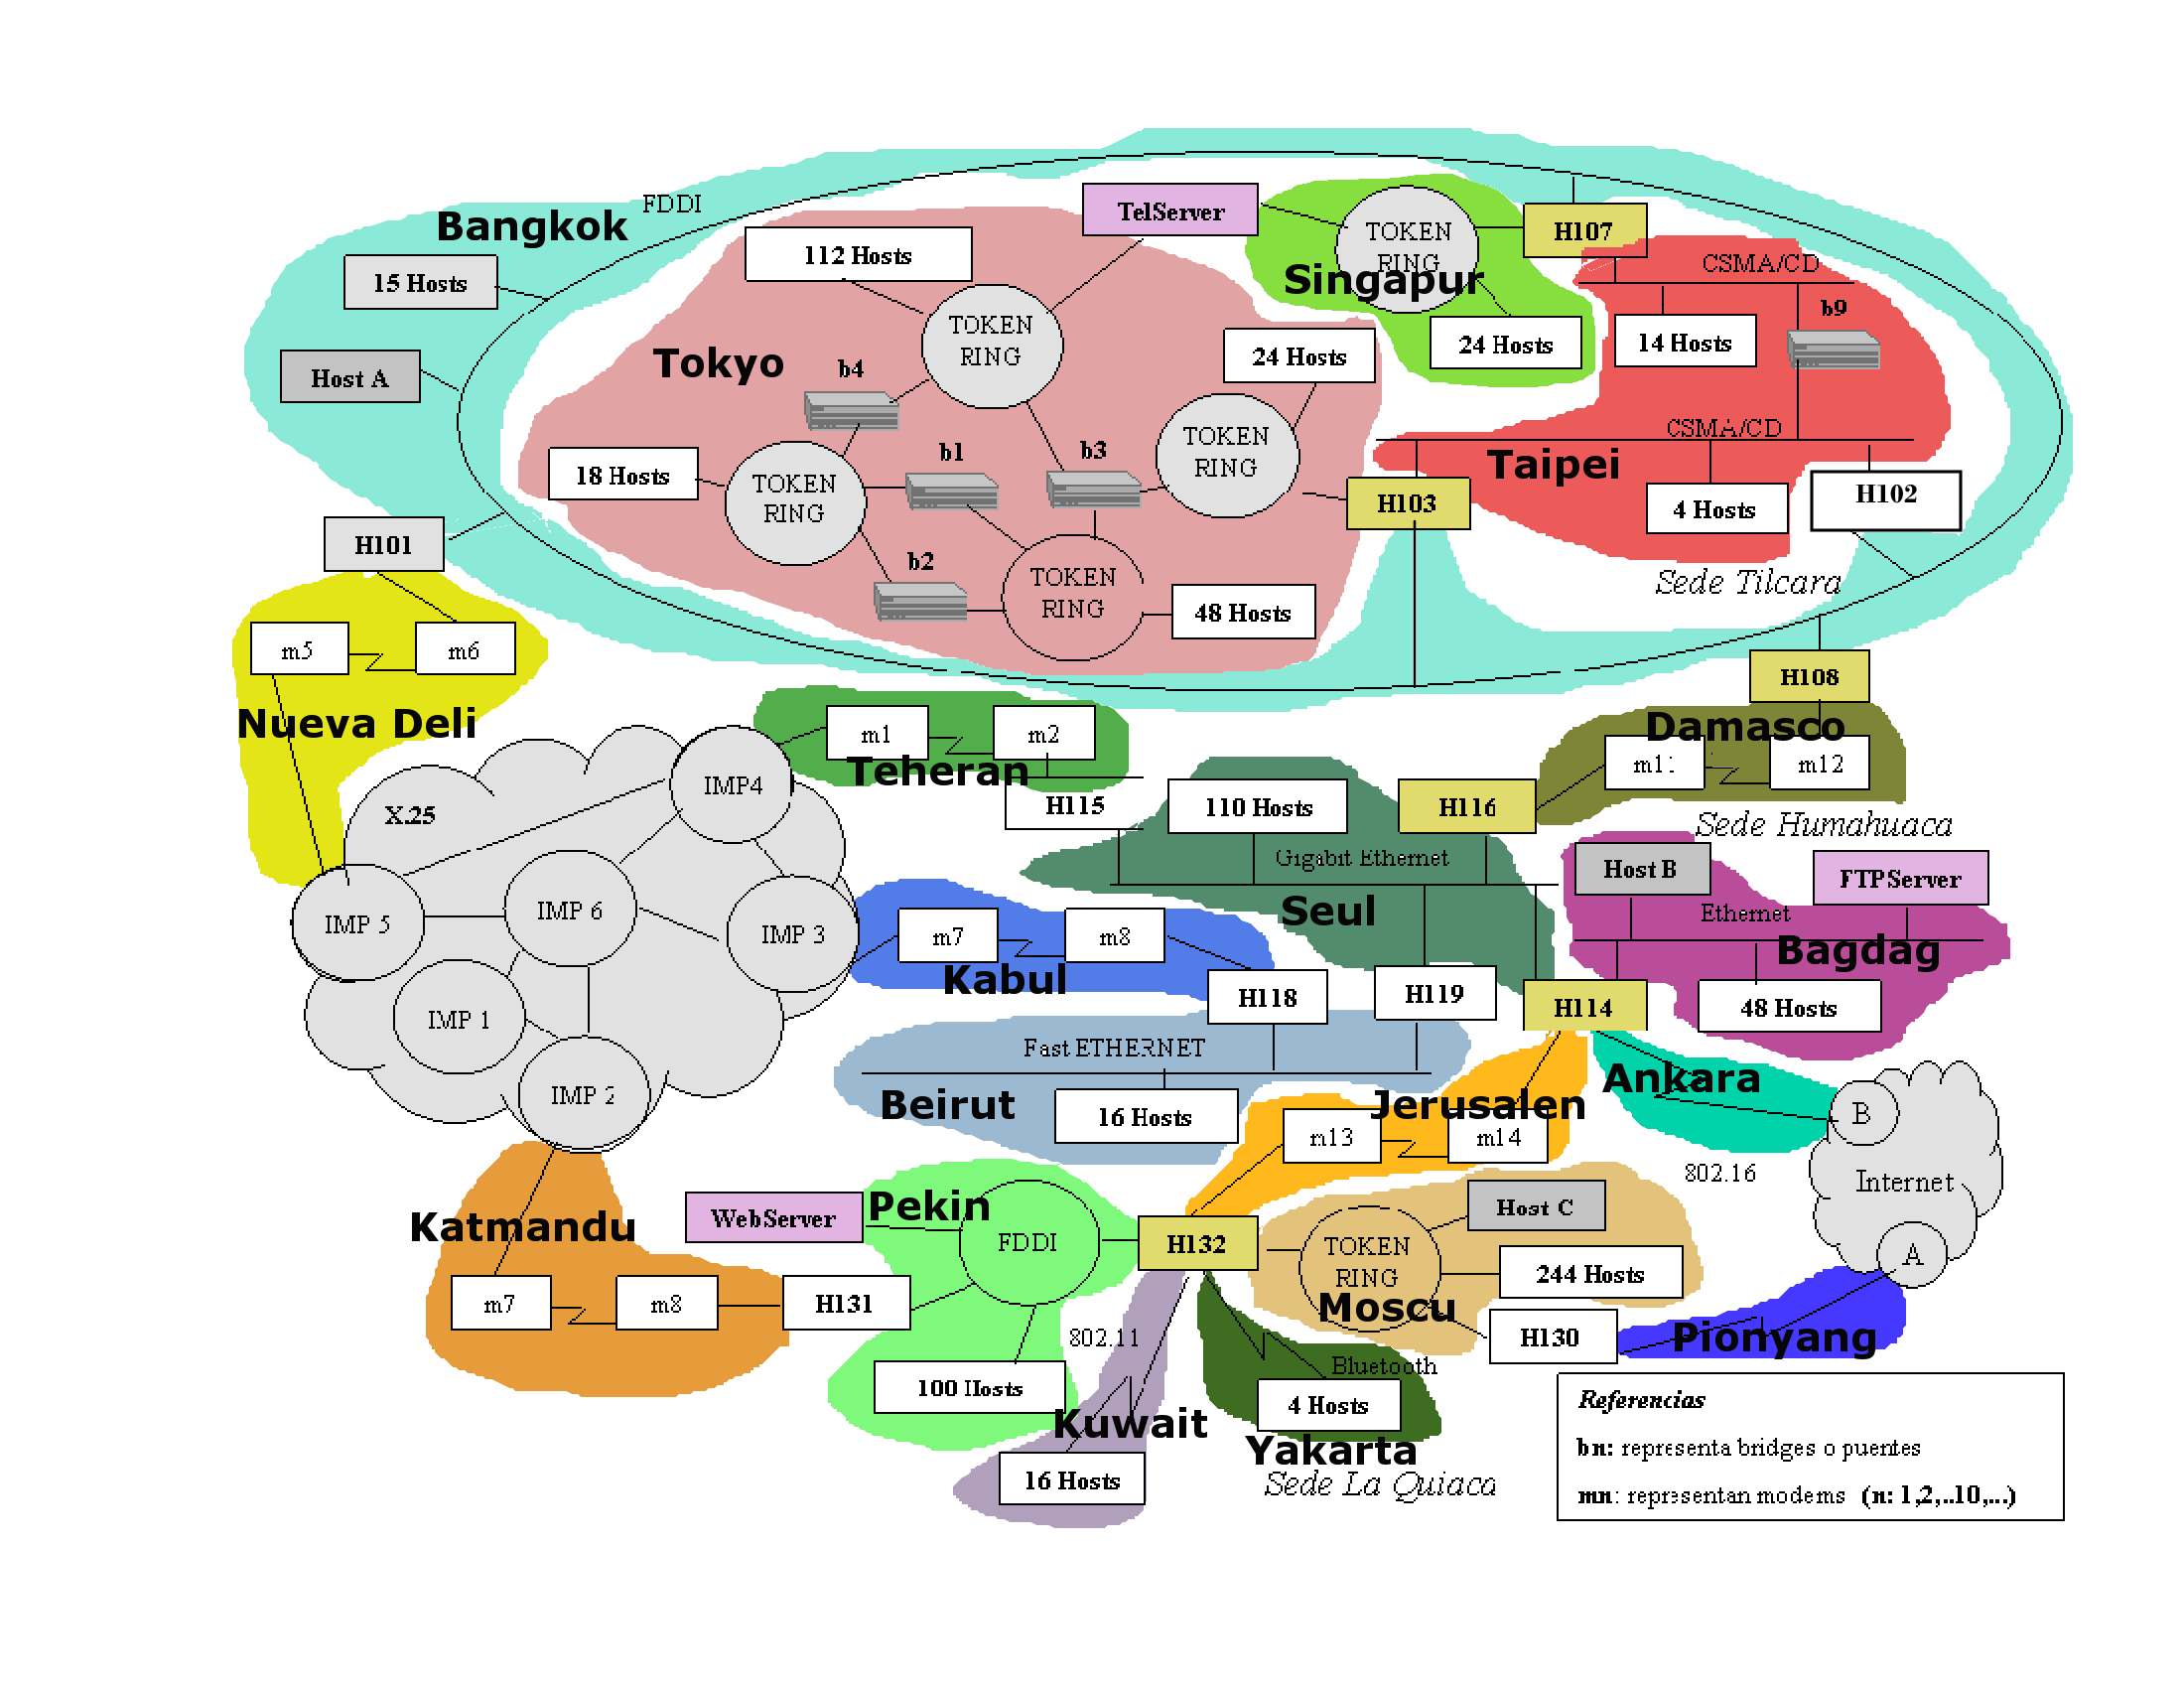
\includegraphics[width=22cm, height=21cm, angle=90]{Subneting.png} \\
  \end{center}
  \caption{Topología de subredes.}
\end{figure}
\FloatBarrier



\section{Tablas de ruteo}

A continuac\'on se incluyen las tablas de ruteo para todos los routers.

\subsection{H101}
\begin{table}
  \begin{center}
    \begin{tabular}{|l|l|l|l|}
      \hline
        \bf{Direcci\'on} & \bf{M\'ascara} & \bf{Gateway} & \bf{M\'etrica} \\
      \hline 
	10.27.15.200  & 255.255.255.252 & 10.39.25.68 & 1 \\
        10.27.15.204  & 255.255.255.252 & 10.39.25.68 & 3 \\
        172.51.5.192  & 255.255.255.252 & 172.51.5.193 & 0 \\
        172.51.5.196  & 255.255.255.252 & 10.39.25.68 & 4 \\
        172.51.5.200  & 255.255.255.252 & 10.39.25.68 & 5 \\
        172.51.5.204  & 255.255.255.252 & 10.39.25.68 & 3 \\
        135.143.5.0   & 255.255.255.252 & 10.39.25.68 & 3 \\
        135.143.5.4   & 255.255.255.252 & 10.39.25.68 & 5 \\ 	
	10.27.15.192  & 255.255.255.248 & 10.39.25.68 & 4 \\
	10.69.6.128   & 255.255.255.224 & 10.39.25.67 & 1 \\
        10.69.6.160   & 255.255.255.224 & 10.39.25.68 & 1 \\
	10.39.25.64   & 255.255.255.224 & 10.39.25.65 & 0 \\       
	10.69.6.224   & 255.255.255.224 & 10.39.25.68 & 3 \\
	10.69.6.192   & 255.255.255.224 & 10.39.25.68 & 4 \\	
	10.39.25.0    & 255.255.255.192 & 10.39.25.68 & 3 \\
	10.39.25.128  & 255.255.255.128 & 10.39.25.68 & 2 \\
	10.42.5.0     & 255.255.255.0 & 10.39.25.68 & 4 \\
        10.69.5.0     & 255.255.255.0 & 10.39.25.66 & 1 \\
        192.168.15.0  & 255.255.255.0 & 10.39.25.68 & 4 \\  
    \hline
    \end{tabular} \\
  \end{center}
  \caption{Tabla de ruteo H101.}
\end{table}
\FloatBarrier

\subsection{H102}
\begin{table}
  \begin{center}
    \begin{tabular}{|l|l|l|l|}
      \hline
        \bf{Direcci\'on} & \bf{M\'ascara} & \bf{Gateway} & \bf{M\'etrica} \\
      \hline 
	10.27.15.200  & 255.255.255.252 & 10.39.25.68 & 1 \\
        10.27.15.204  & 255.255.255.252 & 10.39.25.68 & 3 \\
        172.51.5.192  & 255.255.255.252 & 10.39.25.65 & 1 \\
        172.51.5.196  & 255.255.255.252 & 10.39.25.68 & 4 \\
        172.51.5.200  & 255.255.255.252 & 10.39.25.68 & 5 \\
        172.51.5.204  & 255.255.255.252 & 10.39.25.68 & 3 \\
        135.143.5.0   & 255.255.255.252 & 10.39.25.68 & 3 \\
        135.143.5.4   & 255.255.255.252 & 10.39.25.68 & 5 \\ 	
	10.27.15.192  & 255.255.255.248 & 10.39.25.68 & 4 \\
	10.69.6.128   & 255.255.255.224 & 10.39.25.67 & 1 \\
        10.69.6.160   & 255.255.255.224 & 10.69.6.163 & 0 \\
	10.39.25.64   & 255.255.255.224 & 10.39.25.69 & 0 \\       
	10.69.6.224   & 255.255.255.224 & 10.39.25.68 & 3 \\
	10.69.6.192   & 255.255.255.224 & 10.39.25.68 & 4 \\	
	10.39.25.0    & 255.255.255.192 & 10.39.25.68 & 3 \\
	10.39.25.128  & 255.255.255.128 & 10.39.25.68 & 2 \\
	10.42.5.0     & 255.255.255.0 & 10.39.25.68 & 4 \\
        10.69.5.0     & 255.255.255.0 & 10.39.25.66 & 1 \\
        192.168.15.0  & 255.255.255.0 & 10.39.25.68 & 4 \\  
    \hline
    \end{tabular} \\
  \end{center}
  \caption{Tabla de ruteo H102.}
\end{table}
\FloatBarrier

\subsection{H103}
\begin{table}
  \begin{center}
    \begin{tabular}{|l|l|l|l|}
      \hline
        \bf{Direcci\'on} & \bf{M\'ascara} & \bf{Gateway} & \bf{M\'etrica} \\
      \hline 
	10.27.15.200  & 255.255.255.252 & 10.39.25.68 & 1 \\
        10.27.15.204  & 255.255.255.252 & 10.39.25.68 & 3 \\
        172.51.5.192  & 255.255.255.252 & 10.39.25.65 & 1 \\
        172.51.5.196  & 255.255.255.252 & 10.39.25.68 & 4 \\
        172.51.5.200  & 255.255.255.252 & 10.39.25.68 & 5 \\
        172.51.5.204  & 255.255.255.252 & 10.39.25.68 & 3 \\
        135.143.5.0   & 255.255.255.252 & 10.39.25.68 & 5 \\
        135.143.5.4   & 255.255.255.252 & 10.39.25.68 & 3 \\ 	
	10.27.15.192  & 255.255.255.248 & 10.39.25.68 & 4 \\
	10.69.6.128   & 255.255.255.224 & 10.39.25.67 & 1 \\
        10.69.6.160   & 255.255.255.224 & 10.69.6.161 & 0 \\
	10.39.25.64   & 255.255.255.224 & 10.39.25.66 & 0 \\       
	10.69.6.224   & 255.255.255.224 & 10.39.25.68 & 3 \\
	10.69.6.192   & 255.255.255.224 & 10.39.25.68 & 4 \\	
	10.39.25.0    & 255.255.255.192 & 10.39.25.68 & 3 \\
	10.39.25.128  & 255.255.255.128 & 10.39.25.68 & 2 \\
	10.42.5.0     & 255.255.255.0 & 10.39.25.68 & 4 \\
        10.69.5.0     & 255.255.255.0 & 10.69.5.1 & 0 \\
        192.168.15.0  & 255.255.255.0 & 10.39.25.68 & 4 \\  
    \hline
    \end{tabular} \\
  \end{center}
  \caption{Tabla de ruteo H103.}
\end{table}
\FloatBarrier

\subsection{H107}
\begin{table}
  \begin{center}
    \begin{tabular}{|l|l|l|l|}
      \hline
        \bf{Direcci\'on} & \bf{M\'ascara} & \bf{Gateway} & \bf{M\'etrica} \\
      \hline 
	10.27.15.200  & 255.255.255.252 & 10.39.25.68 & 1 \\
        10.27.15.204  & 255.255.255.252 & 10.39.25.68 & 3 \\
        172.51.5.192  & 255.255.255.252 & 10.39.25.65 & 1 \\
        172.51.5.196  & 255.255.255.252 & 10.39.25.68 & 4 \\
        172.51.5.200  & 255.255.255.252 & 10.39.25.68 & 5 \\
        172.51.5.204  & 255.255.255.252 & 10.39.25.68 & 3 \\
        135.143.5.0   & 255.255.255.252 & 10.39.25.68 & 3 \\
        135.143.5.4   & 255.255.255.252 & 10.39.25.68 & 5 \\ 	
	10.27.15.192  & 255.255.255.248 & 10.39.25.68 & 4 \\
	10.69.6.128   & 255.255.255.224 & 10.69.6.130 & 0 \\
        10.69.6.160   & 255.255.255.224 & 10.69.6.162 & 0 \\
	10.39.25.64   & 255.255.255.224 & 10.39.25.67 & 0 \\       
	10.69.6.224   & 255.255.255.224 & 10.39.25.68 & 3 \\
	10.69.6.192   & 255.255.255.224 & 10.39.25.68 & 4 \\	
	10.39.25.0    & 255.255.255.192 & 10.39.25.68 & 3 \\
	10.39.25.128  & 255.255.255.128 & 10.39.25.68 & 2 \\
	10.42.5.0     & 255.255.255.0 & 10.39.25.68 & 4 \\
        10.69.5.0     & 255.255.255.0 & 10.39.25.66 & 1 \\
        192.168.15.0  & 255.255.255.0 & 10.39.25.68 & 4 \\  
    \hline
    \end{tabular} \\
  \end{center}
  \caption{Tabla de ruteo H107.}
\end{table}
\FloatBarrier


\subsection{H108}
\begin{table}
  \begin{center}
    \begin{tabular}{|l|l|l|l|}
      \hline
        \bf{Direcci\'on} & \bf{M\'ascara} & \bf{Gateway} & \bf{M\'etrica} \\
      \hline 
	10.27.15.200  & 255.255.255.252 & 10.27.15.201 & 0 \\
        10.27.15.204  & 255.255.255.252 & 10.27.15.202 & 2 \\
        172.51.5.192  & 255.255.255.252 & 10.39.25.65 & 1 \\
        172.51.5.196  & 255.255.255.252 & 10.27.15.202 & 3 \\
        172.51.5.200  & 255.255.255.252 & 10.27.15.202 & 4 \\
        172.51.5.204  & 255.255.255.252 & 10.27.15.202 & 2 \\
        135.143.5.0   & 255.255.255.252 & 10.27.15.202 & 2 \\
        135.143.5.4   & 255.255.255.252 & 10.27.15.202 & 4 \\ 	
	10.27.15.192  & 255.255.255.248 & 10.27.15.202 & 3 \\
	10.69.6.128   & 255.255.255.224 & 10.39.25.67 & 1 \\
        10.69.6.160   & 255.255.255.224 & 10.39.25.66 & 1 \\
	10.39.25.64   & 255.255.255.224 & 10.39.25.68 & 0 \\       
	10.69.6.224   & 255.255.255.224 & 10.27.15.202 & 2 \\
	10.69.6.192   & 255.255.255.224 & 10.27.15.202 & 3 \\	
	10.39.25.0    & 255.255.255.192 & 10.27.15.202 & 2 \\
	10.39.25.128  & 255.255.255.128 & 10.27.15.202 & 1 \\
	10.42.5.0     & 255.255.255.0 & 10.27.15.202 & 3 \\
        10.69.5.0     & 255.255.255.0 & 10.39.25.66 & 1 \\
        192.168.15.0  & 255.255.255.0 & 10.27.15.202 & 3 \\  
    \hline
    \end{tabular} \\
  \end{center}
  \caption{Tabla de ruteo H108.}
\end{table}
\FloatBarrier

\subsection{H114}
\begin{table}
  \begin{center}
    \begin{tabular}{|l|l|l|l|}
      \hline
        \bf{Direcci\'on} & \bf{M\'ascara} & \bf{Gateway} & \bf{M\'etrica} \\
      \hline 
	10.27.15.200  & 255.255.255.252 & 10.39.25.131 & 1 \\
        10.27.15.204  & 255.255.255.252 & 10.27.15.205 & 0 \\
        172.51.5.192  & 255.255.255.252 & 10.39.25.131 & 3 \\
        172.51.5.196  & 255.255.255.252 & 10.39.25.132 & 2 \\
        172.51.5.200  & 255.255.255.252 & 10.27.15.206 & 2 \\
        172.51.5.204  & 255.255.255.252 & 10.39.25.130 & 1 \\
        135.143.5.0   & 255.255.255.252 & 135.143.5.1 & 0 \\
        135.143.5.4   & 255.255.255.252 & 10.27.15.206 & 2 \\ 	
	10.27.15.192  & 255.255.255.248 & 10.27.15.206 & 1 \\
	10.69.6.128   & 255.255.255.224 & 10.39.25.131 & 3 \\
        10.69.6.160   & 255.255.255.224 & 10.39.25.131 & 3 \\
	10.39.25.64   & 255.255.255.224 & 10.39.25.131 & 2 \\       
	10.69.6.224   & 255.255.255.224 & 10.39.25.132 & 1 \\
	10.69.6.192   & 255.255.255.224 & 10.27.15.206 & 1 \\	
	10.39.25.0    & 255.255.255.192 & 10.39.25.2 & 0 \\
	10.39.25.128  & 255.255.255.128 & 10.39.25.129 & 0 \\
	10.42.5.0     & 255.255.255.0 & 10.27.15.206 & 1 \\
        10.69.5.0     & 255.255.255.0 & 10.39.25.131 & 3 \\
        192.168.15.0  & 255.255.255.0 & 10.27.15.206 & 1 \\  
    \hline
    \end{tabular} \\
  \end{center}
  \caption{Tabla de ruteo H114.}
\end{table}
\FloatBarrier

\subsection{H115}
\begin{table}
  \begin{center}
    \begin{tabular}{|l|l|l|l|}
      \hline
        \bf{Direcci\'on} & \bf{M\'ascara} & \bf{Gateway} & \bf{M\'etrica} \\
      \hline 
	10.27.15.200  & 255.255.255.252 & 10.39.25.131 & 1 \\
        10.27.15.204  & 255.255.255.252 & 10.39.25.129 & 1 \\
        172.51.5.192  & 255.255.255.252 & 10.39.25.131 & 3 \\
        172.51.5.196  & 255.255.255.252 & 10.39.25.132 & 2 \\
        172.51.5.200  & 255.255.255.252 & 10.39.25.129 & 3 \\
        172.51.5.204  & 255.255.255.252 & 172.51.5.205 & 0 \\
        135.143.5.0   & 255.255.255.252 & 10.39.25.129 & 1 \\
        135.143.5.4   & 255.255.255.252 & 10.39.25.129 & 3 \\ 	
	10.27.15.192  & 255.255.255.248 & 10.39.25.129 & 2 \\
	10.69.6.128   & 255.255.255.224 & 10.39.25.131 & 3 \\
        10.69.6.160   & 255.255.255.224 & 10.39.25.131 & 3 \\
	10.39.25.64   & 255.255.255.224 & 10.39.25.131 & 2 \\       
	10.69.6.224   & 255.255.255.224 & 10.39.25.132 & 1 \\
	10.69.6.192   & 255.255.255.224 & 10.39.25.129 & 1 \\	
	10.39.25.0    & 255.255.255.192 & 10.39.25.129 & 1 \\
	10.39.25.128  & 255.255.255.128 & 10.39.25.130 & 0 \\
	10.42.5.0     & 255.255.255.0 & 10.39.25.129 & 2 \\
        10.69.5.0     & 255.255.255.0 & 10.39.25.131 & 3 \\
        192.168.15.0  & 255.255.255.0 & 10.39.25.129 & 2 \\  
    \hline
    \end{tabular} \\
  \end{center}
  \caption{Tabla de ruteo H115.}
\end{table}
\FloatBarrier

\subsection{H116}
\begin{table}
  \begin{center}
    \begin{tabular}{|l|l|l|l|}
      \hline
        \bf{Direcci\'on} & \bf{M\'ascara} & \bf{Gateway} & \bf{M\'etrica} \\
      \hline 
	10.27.15.200  & 255.255.255.252 & 10.27.15.202 & 0 \\
        10.27.15.204  & 255.255.255.252 & 10.39.25.129 & 1 \\
        172.51.5.192  & 255.255.255.252 & 10.27.15.201 & 2 \\
        172.51.5.196  & 255.255.255.252 & 10.39.25.132 & 2 \\
        172.51.5.200  & 255.255.255.252 & 10.39.25.129 & 3 \\
        172.51.5.204  & 255.255.255.252 & 10.39.25.130 & 1 \\
        135.143.5.0   & 255.255.255.252 & 10.39.25.129 & 3 \\
        135.143.5.4   & 255.255.255.252 & 10.39.25.129 & 3 \\ 	
	10.27.15.192  & 255.255.255.248 & 10.39.25.129 & 2 \\
	10.69.6.128   & 255.255.255.224 & 10.27.15.201 & 2 \\
        10.69.6.160   & 255.255.255.224 & 10.27.15.201 & 2 \\
	10.39.25.64   & 255.255.255.224 & 10.27.15.201 & 2 \\       
	10.69.6.224   & 255.255.255.224 & 10.39.25.132 & 1 \\
	10.69.6.192   & 255.255.255.224 & 10.39.25.129 & 2 \\	
	10.39.25.0    & 255.255.255.192 & 10.39.25.129 & 1 \\
	10.39.25.128  & 255.255.255.128 & 10.39.25.131 & 0 \\
	10.42.5.0     & 255.255.255.0 & 10.39.25.129 & 2 \\
        10.69.5.0     & 255.255.255.0 & 10.27.15.201 & 2 \\
        192.168.15.0  & 255.255.255.0 & 10.39.25.129 & 2 \\  
    \hline
    \end{tabular} \\
  \end{center}
  \caption{Tabla de ruteo H116.}
\end{table}
\FloatBarrier



\subsection{H118}
\begin{table}
  \begin{center}
    \begin{tabular}{|l|l|l|l|}
      \hline
        \bf{Direcci\'on} & \bf{M\'ascara} & \bf{Gateway} & \bf{M\'etrica} \\
      \hline 
	10.27.15.200  & 255.255.255.252 & 10.69.6.226 & 2 \\
        10.27.15.204  & 255.255.255.252 & 10.69.6.226 & 2 \\
        172.51.5.192  & 255.255.255.252 & 10.69.6.226 & 4 \\
        172.51.5.196  & 255.255.255.252 & 172.51.5.197 & 0 \\
        172.51.5.200  & 255.255.255.252 & 10.69.6.226 & 4 \\
        172.51.5.204  & 255.255.255.252 & 10.69.6.226 & 2 \\
        135.143.5.0   & 255.255.255.252 & 10.69.6.226 & 2 \\
        135.143.5.4   & 255.255.255.252 & 10.69.6.226 & 4 \\ 	
	10.27.15.192  & 255.255.255.248 & 10.69.6.226 & 3 \\
	10.69.6.128   & 255.255.255.224 & 10.69.6.226 & 4 \\
        10.69.6.160   & 255.255.255.224 & 10.69.6.226 & 4 \\
	10.39.25.64   & 255.255.255.224 & 10.69.6.226 & 3 \\       
	10.69.6.224   & 255.255.255.224 & 10.69.6.225 & 0 \\
	10.69.6.192   & 255.255.255.224 & 10.69.6.226 & 3 \\	
	10.39.25.0    & 255.255.255.192 & 10.69.6.226 & 2 \\
	10.39.25.128  & 255.255.255.128 & 10.69.6.226 & 1 \\
	10.42.5.0     & 255.255.255.0 & 10.69.6.226 & 3 \\
        10.69.5.0     & 255.255.255.0 & 10.69.6.226 & 4 \\
        192.168.15.0  & 255.255.255.0 & 10.69.6.226 & 3 \\  
    \hline
    \end{tabular} \\
  \end{center}
  \caption{Tabla de ruteo H118.}
\end{table}
\FloatBarrier

\subsection{H119}
\begin{table}
  \begin{center}
    \begin{tabular}{|l|l|l|l|}
      \hline
        \bf{Direcci\'on} & \bf{M\'ascara} & \bf{Gateway} & \bf{M\'etrica} \\
      \hline 
	10.27.15.200  & 255.255.255.252 & 10.39.25.131 & 1 \\
        10.27.15.204  & 255.255.255.252 & 10.39.25.129 & 1 \\
        172.51.5.192  & 255.255.255.252 & 10.39.25.131 & 3 \\
        172.51.5.196  & 255.255.255.252 & 10.69.6.225 & 1 \\
        172.51.5.200  & 255.255.255.252 & 10.39.25.129 & 3 \\
        172.51.5.204  & 255.255.255.252 & 10.39.25.130 & 1 \\
        135.143.5.0   & 255.255.255.252 & 10.39.25.129 & 1 \\
        135.143.5.4   & 255.255.255.252 & 10.39.25.129 & 3 \\ 	
	10.27.15.192  & 255.255.255.248 & 10.39.25.129 & 2 \\
	10.69.6.128   & 255.255.255.224 & 10.39.25.131 & 3 \\
        10.69.6.160   & 255.255.255.224 & 10.39.25.131 & 3 \\
	10.39.25.64   & 255.255.255.224 & 10.39.25.131 & 2 \\       
	10.69.6.224   & 255.255.255.224 & 10.69.6.226 & 0 \\
	10.69.6.192   & 255.255.255.224 & 10.39.25.129 & 2 \\	
	10.39.25.0    & 255.255.255.192 & 10.39.25.129 & 1 \\
	10.39.25.128  & 255.255.255.128 & 10.39.25.132 & 0 \\
	10.42.5.0     & 255.255.255.0 & 10.39.25.129 & 2 \\
        10.69.5.0     & 255.255.255.0 & 10.39.25.131 & 3 \\
        192.168.15.0  & 255.255.255.0 & 10.39.25.129 & 2 \\  
    \hline
    \end{tabular} \\
  \end{center}
  \caption{Tabla de ruteo H119.}
\end{table}
\FloatBarrier

\subsection{H130}
\begin{table}
  \begin{center}
    \begin{tabular}{|l|l|l|l|}
      \hline
        \bf{Direcci\'on} & \bf{M\'ascara} & \bf{Gateway} & \bf{M\'etrica} \\
      \hline 
	10.27.15.200  & 255.255.255.252 & 10.42.5.2 & 3 \\
        10.27.15.204  & 255.255.255.252 & 10.42.5.2 & 1 \\
        172.51.5.192  & 255.255.255.252 & 10.42.5.2 & 5 \\
        172.51.5.196  & 255.255.255.252 & 10.42.5.2 & 4 \\
        172.51.5.200  & 255.255.255.252 & 10.42.5.2 & 2 \\
        172.51.5.204  & 255.255.255.252 & 10.42.5.2 & 3 \\
        135.143.5.0   & 255.255.255.252 & 10.42.5.2 & 2 \\
        135.143.5.4   & 255.255.255.252 & 135.143.5.5 & 0 \\ 	
	10.27.15.192  & 255.255.255.248 & 10.42.5.2 & 1 \\
	10.69.6.128   & 255.255.255.224 & 10.42.5.2 & 5 \\
        10.69.6.160   & 255.255.255.224 & 10.42.5.2 & 5 \\
	10.39.25.64   & 255.255.255.224 & 10.42.5.2 & 4 \\       
	10.69.6.224   & 255.255.255.224 & 10.42.5.2 & 3 \\
	10.69.6.192   & 255.255.255.224 & 10.42.5.2 & 1 \\	
	10.39.25.0    & 255.255.255.192 & 10.42.5.2 & 2 \\
	10.39.25.128  & 255.255.255.128 & 10.42.5.2 & 2 \\
	10.42.5.0     & 255.255.255.0 & 10.42.5.1 & 0 \\
        10.69.5.0     & 255.255.255.0 & 10.42.5.2 & 5 \\
        192.168.15.0  & 255.255.255.0 & 10.42.5.2 & 1 \\  
    \hline
    \end{tabular} \\
  \end{center}
  \caption{Tabla de ruteo H130.}
\end{table}
\FloatBarrier

\subsection{H131}
\begin{table}
  \begin{center}
    \begin{tabular}{|l|l|l|l|}
      \hline
        \bf{Direcci\'on} & \bf{M\'ascara} & \bf{Gateway} & \bf{M\'etrica} \\
      \hline 
	10.27.15.200  & 255.255.255.252 & 192.168.15.2 & 3 \\
        10.27.15.204  & 255.255.255.252 & 192.168.15.2 & 1 \\
        172.51.5.192  & 255.255.255.252 & 192.168.15.2 & 5 \\
        172.51.5.196  & 255.255.255.252 & 192.168.15.2 & 4 \\
        172.51.5.200  & 255.255.255.252 & 172.51.5.201 & 0 \\
        172.51.5.204  & 255.255.255.252 & 192.168.15.2 & 3 \\
        135.143.5.0   & 255.255.255.252 & 192.168.15.2 & 2 \\
        135.143.5.4   & 255.255.255.252 & 192.168.15.2 & 2 \\ 	
	10.27.15.192  & 255.255.255.248 & 192.168.15.2 & 1 \\
	10.69.6.128   & 255.255.255.224 & 192.168.15.2 & 5 \\
        10.69.6.160   & 255.255.255.224 & 192.168.15.2 & 5 \\
	10.39.25.64   & 255.255.255.224 & 192.168.15.2 & 4 \\       
	10.69.6.224   & 255.255.255.224 & 192.168.15.2 & 3 \\
	10.69.6.192   & 255.255.255.224 & 192.168.15.2 & 1 \\	
	10.39.25.0    & 255.255.255.192 & 192.168.15.2 & 2 \\
	10.39.25.128  & 255.255.255.128 & 192.168.15.2 & 2 \\
	10.42.5.0     & 255.255.255.0 & 192.168.15.2 & 1 \\
        10.69.5.0     & 255.255.255.0 & 192.168.15.2 & 5 \\
        192.168.15.0  & 255.255.255.0 & 192.168.15.3 & 0 \\  
    \hline
    \end{tabular} \\
  \end{center}
  \caption{Tabla de ruteo H131.}
\end{table}
\FloatBarrier


\subsection{H132}
\begin{table}
  \begin{center}
    \begin{tabular}{|l|l|l|l|}
      \hline
        \bf{Direcci\'on} & \bf{M\'ascara} & \bf{Gateway} & \bf{M\'etrica} \\
      \hline 
	10.27.15.200  & 255.255.255.252 & 10.27.15.205 & 2 \\
        10.27.15.204  & 255.255.255.252 & 10.27.15.206 & 0 \\
        172.51.5.192  & 255.255.255.252 & 10.27.15.205 & 4 \\
        172.51.5.196  & 255.255.255.252 & 10.27.15.205 & 3 \\
        172.51.5.200  & 255.255.255.252 & 192.168.15.3 & 1 \\
        172.51.5.204  & 255.255.255.252 & 10.27.15.205 & 2 \\
        135.143.5.0   & 255.255.255.252 & 10.27.15.205 & 1 \\
        135.143.5.4   & 255.255.255.252 & 10.42.5.1 & 1 \\ 	
	10.27.15.192  & 255.255.255.248 & 10.27.15.193 & 0 \\
	10.69.6.128   & 255.255.255.224 & 10.27.15.205 & 4 \\
        10.69.6.160   & 255.255.255.224 & 10.27.15.205 & 4 \\
	10.39.25.64   & 255.255.255.224 & 10.27.15.205 & 3 \\       
	10.69.6.224   & 255.255.255.224 & 10.27.15.205 & 2 \\
	10.69.6.192   & 255.255.255.224 & 10.69.6.193 & 0 \\	
	10.39.25.0    & 255.255.255.192 & 10.27.15.205 & 1 \\
	10.39.25.128  & 255.255.255.128 & 10.27.15.205 & 1 \\
	10.42.5.0     & 255.255.255.0 & 10.42.5.2 & 0 \\
        10.69.5.0     & 255.255.255.0 & 10.27.15.205 & 4 \\
        192.168.15.0  & 255.255.255.0 & 192.168.15.2 & 0 \\  
    \hline
    \end{tabular} \\
  \end{center}
  \caption{Tabla de ruteo H132.}
\end{table}
\FloatBarrier




\subsection{Rutas alternativas}




\section{DNS}
La configuración de los servidores DNS, según lo indicado en el enunciado del trabajo práctico, debe realizarse utilizando un DNS root, de nivel 1, y dos DNS de nivel 2. 
El DNS de nivel 1 se encarga de hacer forward entre los DNS de nivel 2, es decir, deriva las consultas al DNS correspondiente.
Los DNS de nivel 2 son los encargados de resolver las consultas entre los distintos hosts.
Los servidores deben poder resolver tanto consultas directas (preguntando por un dominio y devolviendo la ip correspondiente a ese dominio) como reversas (preguntando por una ip y devolviendo el nombre del dominio que tiene esa ip).
Los servidores que tenemos son:
	- root en H116
	- 1 de nivel 2 en H102 para la sede Tilcara
	- 1 de nivel 2 en H132 para el resto de las sedes, Humahuaca y La Quiaca

El H102 además de resolver las consultas para los hosts que estén dentro de las subredes en la sede Tilcara, también va a tener el servidor telnet.
El H132 además de resolver las consultas para los hosts que estén dentro de las subredes en las sedes Humahuaca y La Quiaca, también va a tener los servidores web y ftp.


Utilizamos el BIND9 para emular un DNS en una pc.

Todos los equipos que necesiten comunicarse con otros, lo harán a través del root, el cual derivará al DNS correspondiente según la sede donde se encuentre el host destino.

En caso que el DNS root no esté activo, no se podrán realizar consultas entre las sedes Tilcara y resto (Humahuaca y La Quiaca) ya que el DNS root es el que conecta a ambos DNS de nivel 2.
Del mismo modo, si alguno de los DNS de nivel 2 no están activos, tampoco se podrán realizar consultas entre ambas sedes.

Para levantar un DNS en una máquina, hay que correr el script ./install-dns.sh y pasarle como parámetro:
	root-dns ----->	si se quiere levantar el DNS root
	tilcara-dns --> si se quiere levantar el DNS para la sede Tilcara
	resto-dns ---->	si se quiere levantar el DNS para las sedes Humahuaca y La Quiaca

\section{Simulación en la sala}

\section{Conclusiones}


% ------------------------------ Bibliografía -------------------------------

\newpage

\begin{thebibliography}{9}

\bibitem{rfc950}
  \emph{RFC 950 - Internet Standard Subnetting Procedure}. \\
  http://www.packetizer.com/rfc/rfc950/

\end{thebibliography}


% ------------------------------ Fin del tp -------------------------------

\end{document}

%---------------------------- Fin del documento ---------------------------
